\documentclass{article} % Класс печатного документа

% для поддержки русского языка
\usepackage[T2A]{fontenc} % поддержка специальных русских символов
\usepackage[utf8]{inputenc} % Кодировка исходного текста - utf8
\usepackage[english,russian]{babel} % Поддержка языка - русского с английским
\usepackage{indentfirst} % Отступ в первом абзаце

\usepackage{graphicx} % Для вставки картинок
\usepackage{hyperref} % Для вставки гиперссылок
\usepackage{listings} % Для вставки кусков кода
\usepackage{float} % Для точного позиционирования картинок
\usepackage{amsmath} % Для отключения нумерации у указанных формул
\usepackage{listings} % Добавление листингов
\usepackage[justification=centering]{caption} % для центрирования подписи к таблице

\title{Отчёт 2\\
Исследование поведения медианы и усечённого среднего\\
для загрязнённого нормального распределения} % заголовок документа
\author{Свичкарев А.\,В.} % Автор документа
\date{\today} % Текущая дата

\begin{document} % Конец преамбулы, начало текста

\maketitle % Печатает заголовок, список авторов и дату

\section*{Задачи}
Рассмотрим два вида распределений:
\begin{itemize}
    \item Нормальное распределение N(x;y);
    \item Смесь нормальных распределений вида: $0.9 N(x;0,1) + 0.1 N(x;0,3)$.
\end{itemize}

Как и раньше рассмотрим три объема выборок из данных распределений:
10, 20, 100. 
\bigskip

Рассчитать для данных выборок основные параметры:
\begin{enumerate}
    \item Медиану;
    \item Усечённое среднее
        (для разных значений $\alpha = 0.05, 0.1, 0.15, 0.2, 0.25$).
\end{enumerate}

Для смеси нормальных распределений вида:

\begin{equation*}
(1-epsilon) \cdot N(x;1,0) + epsilon \cdot N(x;1000,0)
\end{equation*}
проверить достижение максимально возможного значения
пороговой точки медианы при $epsilon = 0.5$
и найти значение $epsilon$,
при котором достигается максимально возможное значение
пороговой точки $alpha$-усеченного среднего
для разных значений
$alpha = 0.05, 0.1, 0.15, 0.2, 0.25$.

\section*{Выполнение}

На следующей таблице представлены результаты вычислений
основных параметров:

\begin{table}[H]
\centering
\begin{tabular}{|c|c|c|c|}
\hline
\textbf{volume} & \textbf{alpha} & \textbf{median} & \textbf{trMean} \\ \hline
10              & 0.05           & -0.05365556     & -0.04452626     \\ \hline
10              & 0.1            & 0.003579504     & -0.02463174     \\ \hline
10              & 0.15           & 0.05596931      & 0.06307632      \\ \hline
10              & 0.2            & -0.001088526    & -0.0001511442   \\ \hline
10              & 0.25           & 0.007665013     & 0.0006324276    \\ \hline
20              & 0.05           & 0.04777282      & 0.01150508      \\ \hline
20              & 0.1            & 0.007970752     & 0.009856205     \\ \hline
20              & 0.15           & 0.03416975      & 0.02412901      \\ \hline
20              & 0.2            & -0.02134803     & -0.03098677     \\ \hline
20              & 0.25           & 0.02447365      & 0.02951892      \\ \hline
100             & 0.05           & 0.004489417     & -0.0004347693   \\ \hline
100             & 0.1            & 0.008021296     & 0.004741634     \\ \hline
100             & 0.15           & -0.01361388     & -0.01546016     \\ \hline
100             & 0.2            & 0.01054349      & 0.001793458     \\ \hline
100             & 0.25           & -0.0001443635   & -0.00649204     \\ \hline
\end{tabular}
\caption{Значения медианы и усечённого среднего
для различных комбинаций параметров}
\end{table}

При увеличение размера выборки значение медианы
и усечённого среднего стремится к мат.ожиданию
генеральной совокупности.
При увеличение $alpha$ значение усечённого среднего
стремится к мат.ожиданию генеральной совокупности,
так как меньше выбросов влияют на значения.

\clearpage
Поиск значения $epsilon$ при пороговой точке:
\begin{figure}[H]
    \centering
    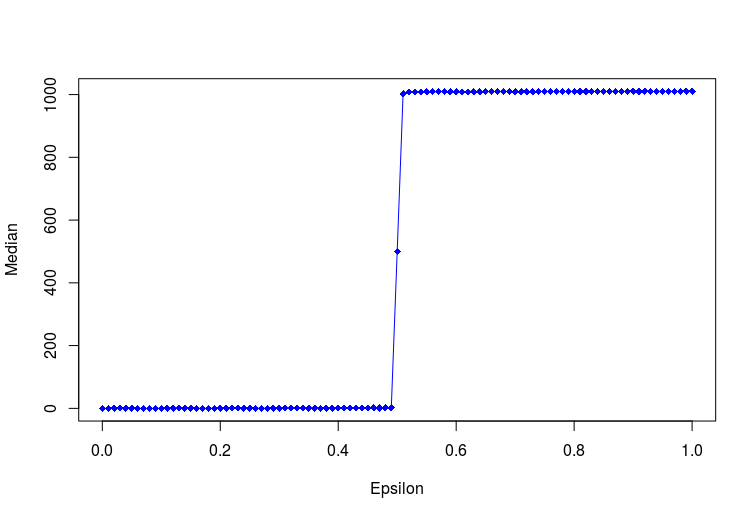
\includegraphics[width=\textwidth]{median}
    \caption{Зависимость значения медианы от количества примесей}
\end{figure}

\begin{figure}[H]
    \centering
    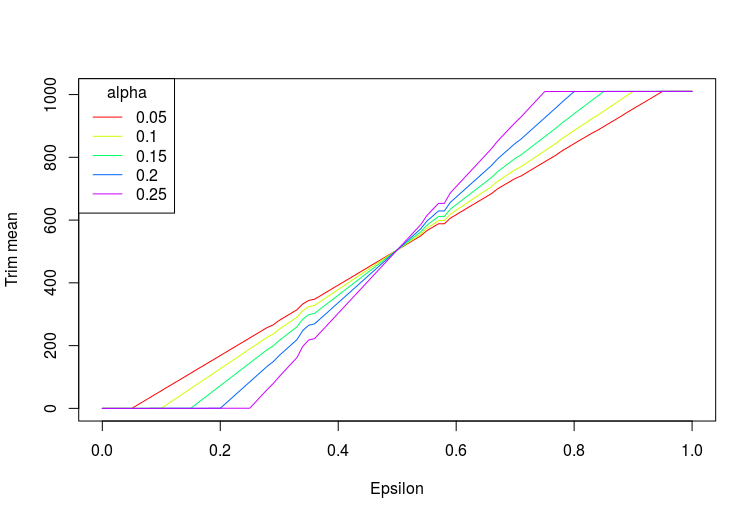
\includegraphics[width=\textwidth]{trimmean}
    \caption{Зависимость значения усечённого среднего
    от количества примесей при различных значениях $alpha$}
\end{figure}

При значение $epsilon = 0.5$
достигается максимальное значение пороговой точки.
Медиана хорошо реагирует на
переход с большей части одного распределения
на большую часть другого распределения.

Усечённое среднее плавно переходит
между мат.ожиданиями двух распределений.
Чем больше $alpha$,
тем больше наклон в средней части и
большая нечувствительность к
маленьким примесям другого распределения.
Предельный наклон достигается в медиане,
так как её можно рассматривать как усечённое среднее
при $alpha = 0.5$.

\section*{Исходный код}
Исходный код прилагается.

\end{document} % Конец документа
